\section{Introduction}
\label{sec:intro}

This report mainly deals with Non-Equilibrium flows in general and how different they are from chemical and local Equilibrium, For example, Assuming Chemical and Local Equilibrium effects are present, In a convergent divergent nozzle, the flow at the throat is choked, that means the throat Mach Number = 1, where as in Non-Equilibrium flow that is not the case, Oblique shocks for example, the shock tend to be straight in Local and Chemical Equilibrium where as in it tends to bend in Non Equilibrium flows. Non Equilibrium flows basically changes the main physical and governing equation that are associated in predicting the flow features. This present chapter or report completely describes what are the changes in the flow features changes that are encountered while solving the equations.

\hspace{1cm}


For any  High Temperature or Hypersonic flows prediction of the flow property effects without actually testing or performing physical tasks whether it is by wind tunnels or computational fluid dynamic, but rather by the use of analytical or visualization methods would be recommended for such complex flow scenarios.

\hspace{1cm}
 
To study about such complex flow scenarios, we first need to understand the prerequisites of the flow features, that is

\vspace{1cm}
Frozen flow: which basically means the net reaction rate is zero, or simple words, the temperature of the flow that is generated does not effect the molecules of the gas and hence the molecules in the temperature retain their integrity of their state which indirectly points that the relaxation time or the vibrational relaxation time of the molecules is very high 


\vspace{1cm}
In frozen flows, there is absolutely no reaction, just a chunk of fluid or inert fluid moving around the flowfield and the molecules tend to have higher relaxation times
\vspace{1cm}


Equilibrium flows: This flow scenarios occur when the flow reaction rates, that is forward and backward reaction rates tend to go very large number in-turn reducing the vibrational relaxation time of the molecules to be zero

\vspace{1cm}

To elaborate this even more, assume the flowfield that is present which mainly governed by pressure and temperature changes with respect to space and time, now in order to obtain an equilibrium flow, the internal energy modes and the chemical composition of the local equilibrium values must maintain or adjust instantly with the change in flow conditions, that means the fluid must be reactive, reactive to the level where the reaction rates that are present in the flow must tend to infinity and the vibrational relaxation time tend to zero, such type of flows are equilibrium flows. 
\vspace{1cm}

The road map for the current chapter depicted in Figure 1, have 7 parts to deal with, starting with introduction of Inviscid High temperature Non Equilibrium flows, Governing equation that control and predict the flow features analytically, Applying he governing equations to shock waves and other supersonic quantities and nozzle flows and observe how the flow features comparatively change in non-equilibrium case when compared to equilibrium case. Blunt Body case and Binary scaling of the flow and finally study about Non-Equilibrium method of characteristics.

The below figure depicts the outline and road map for the following report.


\begin{figure}
\centering
  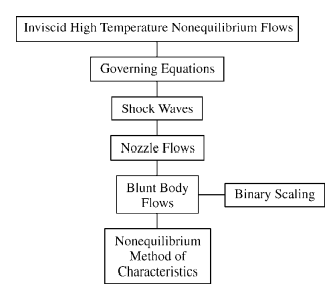
\includegraphics[width=0.5\linewidth]{images/roadmap.png}
  \caption{Road map for Non-Equilibrium flows}
  \label{fig:boat1}
\end{figure}


%This is how to use the references~\cite{Berndtsson607210, Blomkvist2014} or~\cite{Turing1950}.



